
% ----------------------------------------------------------------------
%  Set the document class
% ----------------------------------------------------------------------
\documentclass[11pt,a4paper,twoside]{article}

% ----------------------------------------------------------------------
% Define external packages, language, margins, fonts and new commands
% ----------------------------------------------------------------------
%\input{preamble} 
\usepackage[utf8]{inputenc}   % <<<<< Linux
\usepackage[english]{babel} % <<<<< English
\usepackage{notoccite}
\usepackage[skip=0.5\baselineskip]{caption}
\hyphenation{GTKWave}
\usepackage{listings}
\usepackage[all]{nowidow}

%blind text
\usepackage{lipsum}

\usepackage{graphicx}
\graphicspath{ {./} {../../figlib/} }
\def\FontLn{% 16 pt normal
  \usefont{T1}{phv}{m}{n}\fontsize{16pt}{16pt}\selectfont}
\def\FontLb{% 16 pt bold
  \usefont{T1}{phv}{b}{n}\fontsize{16pt}{16pt}\selectfont}
\def\FontMn{% 14 pt normal
  \usefont{T1}{phv}{m}{n}\fontsize{14pt}{14pt}\selectfont}
\def\FontMb{% 14 pt bold
  \usefont{T1}{phv}{b}{n}\fontsize{14pt}{14pt}\selectfont}
\def\FontSn{% 12 pt normal
  \usefont{T1}{phv}{m}{n}\fontsize{12pt}{12pt}\selectfont}

% Use Arial font as default
%
\renewcommand{\rmdefault}{phv}
\renewcommand{\sfdefault}{phv}
\usepackage{geometry}	
\geometry{verbose,tmargin=2.5cm,bmargin=2.5cm,lmargin=2.5cm,rmargin=2.5cm}

%\usepackage{setspace}
%\renewcommand{\baselinestretch}{1.5}

\usepackage[pdftex]{hyperref} % enhance documents that are to be
                              % output as HTML and PDF
\hypersetup{colorlinks,       % color text of links and anchors,
                              % eliminates borders around links
%            linkcolor=red,    % color for normal internal links
            linkcolor=black,  % color for normal internal links
            anchorcolor=black,% color for anchor text
%            citecolor=green,  % color for bibliographical citations
            citecolor=black,  % color for bibliographical citations
%            filecolor=magenta,% color for URLs which open local files
            filecolor=black,  % color for URLs which open local files
%            menucolor=red,    % color for Acrobat menu items
            menucolor=black,  % color for Acrobat menu items
%            pagecolor=red,    % color for links to other pages
            pagecolor=black,  % color for links to other pages
%            urlcolor=cyan,    % color for linked URLs
            urlcolor=black,   % color for linked URLs
	          bookmarks=true,         % create PDF bookmarks
	          bookmarksopen=false,    % don't expand bookmarks
	          bookmarksnumbered=true, % number bookmarks
	          pdftitle={report},
            pdfauthor={Andre C. Marta},
%            pdfsubject={Thesis Title},
%            pdfkeywords={Thesis Keywords},
            pdfstartview=FitV,
            pdfdisplaydoctitle=true}

\usepackage[numbers,sort&compress]{natbib} % <<<<< References in numbered list [1],[2],...
\usepackage{subcaption} 
\usepackage{mdframed}
\usepackage{amsmath}

%%%%%%%%%%%%%%%%%%%%%%%%%%%%%%%%%%%%%%%%%%%%%%%%%%%%%%%%%%%%%%%%%%%%%%%%
%     Begin Document                                                   %
%%%%%%%%%%%%%%%%%%%%%%%%%%%%%%%%%%%%%%%%%%%%%%%%%%%%%%%%%%%%%%%%%%%%%%%%


\begin{document}

% Set plain page style (no headers, footer with centered page number)
\pagestyle{plain}

% Set roman numbering (i,ii,...) before the start of chapters
%\pagenumbering{roman}

% ----------------------------------------------------------------------
%  Cover page
% ----------------------------------------------------------------------
%%%%%%%%%%%%%%%%%%%%%%%%%%%%%%%%%%%%%%%%%%%%%%%%%%%%%%%%%%%%%%%%%%%%%%%%
%                                                                      %
%     File: Thesis_FrontCover.tex                                      %
%     Tex Master: Thesis.tex                                           %
%                                                                      %
%     Author: Andre C. Marta                                           %
%     Last modified :  2 Jul 2015                                      %
%                                                                      %
%%%%%%%%%%%%%%%%%%%%%%%%%%%%%%%%%%%%%%%%%%%%%%%%%%%%%%%%%%%%%%%%%%%%%%%%

\thispagestyle {empty}

% IST Logo - Signature A
% parameters: bb=llx lly urx ury (bounding box), width=h_length, height=v_length, angle=angle, scale=factor, clip=true/false, draft=true/false. 
\includegraphics[bb=9.5cm 11cm 0cm 0cm,scale=0.29]{IST_A_CMYK_POS}

\begin{center}
%
% Figure (Image or plot)
\vspace{1.0cm}
% height = 50 mm
%\includegraphics[height=50mm]{Figures/Airbus_A350.jpg}

% Title, author and degree
\vspace{1cm}
{\FontLb Circuit Theory and Electronics Fundamentals} \\ % <<<<< EDIT TITLE
\vspace{1cm}
{\FontSn MEAer (Integrated Master In Aerospace Engineering), Técnico, University of Lisbon} \\ % <<<<< EDIT COURSE
\vspace{1cm}
{\FontSn Laboratory 4: Audio Amplifier Circuit} \\
\vspace{1cm}
{\FontSn Group 3} \\
\vspace{0.7cm}
{\FontSn Diogo Faustino, nº95782} \\
\vspace{0.4mm}
{\FontSn Henry Machado, nº95795} \\
\vspace{0.4mm}
{\FontSn Rúben Novais, nº95843} \\
\vspace{1cm}
{\FontSn May 23, 2021} \\ % <<<<< EDIT DATE (corresponds to date of oral examination)
%
\end{center}



% ----------------------------------------------------------------------
% Dedication page (optional)
% ----------------------------------------------------------------------
%\input{dedication} 
%\cleardoublepage

% ----------------------------------------------------------------------
%  Acknowledgments (optional)
% ----------------------------------------------------------------------
%\input{acknowledgements}
%\cleardoublepage

% ----------------------------------------------------------------------
%  Abstract (both in English and Portuguese)
% ----------------------------------------------------------------------
%\input{resumo} 
%\cleardoublepage

%\input{abstract} 

% ----------------------------------------------------------------------
%  Table of contents, list of tables, list of figures and nomenclature
% ----------------------------------------------------------------------

% Table of contents
%
\tableofcontents

% List of tables
%\addcontentsline{toc}{section}{\listtablename}
%\listoftables
%\cleardoublepage 

% List of figures
%\addcontentsline{toc}{section}{\listfigurename}
%\listoffigures
%\cleardoublepage 

% Set arabic numbering (1,2,...) after preface
%
%\setcounter{page}{1}
%\pagenumbering{arabic}

% ----------------------------------------------------------------------
%  Body
% ----------------------------------------------------------------------

\section{Introduction}
\label{sec:introduction}
% state the learning objective 
The objective of this laboratory assignment is to study the behaviour of an RC circuit powered by a sinusoidal voltage source $V_{s}$, as seen in Figure~\ref{fig:rc}. In order to analyse it, we will make use of different techniques such as Thevenin and Phasor analysis in order to establish the natural, forced and total solutions of the circuit. A frequency response analysis then follows, where we look at the magnitude and phase as a function of frequency. Then, we compare the theoretical and simulation data.

In Section~\ref{sec:analysis}, we go through the various steps that are needed to obtain the total solution of the circuit (natural plus forced responses) and present the theoretical frequency response analysis.
In Section~\ref{sec:simulation}, we present the circuit response as simulated in NGSpice. The results in operating point, transient analysis and frequency analysis are compared to the theoretical results obtained in Section~\ref{sec:analysis} and the conclusions of this study are laid out in
Section~\ref{sec:conclusion}.

\begin{figure}[h] \centering
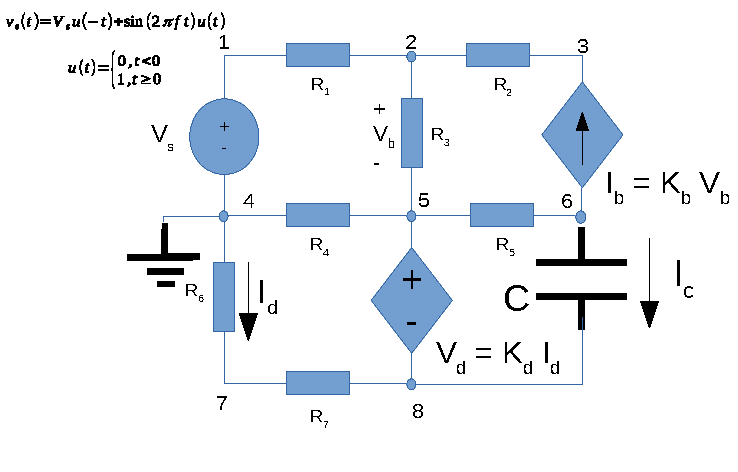
\includegraphics[width=0.9\linewidth]{rc.pdf}
\caption{RC circuit.}
\label{fig:rc}
\end{figure}



\section{Theoretical Analysis}
\label{sec:analysis}
First of all, we performed an operating point analysis in order to check if the transistor was operating in the forward active region.
\begin{table}[h!]
  \centering
  \begin{tabular}{|l|r|}
    \hline    
    {\bf Name} & {\bf Values} \\ \hline
    \input{th_data_tab} 
  \end{tabular}
  \caption{Operating point analysis results.}
  \label{tab:data}
\end{table}

As we can see, VCE is greater than VBEON (0.7V), so we're good to go.
\subsection{Gain Stage}
For the gain stage, the analysis of the incremental circuit yielded the following results:
\begin{table}[h]
  \centering
  \begin{tabular}{|l|r|}
    \hline    
    {\bf Name} & {\bf Values [V]} \\ \hline
    \input{gain_tab} 
  \end{tabular}
  \caption{Gain stage theoretical results}
  \label{tab:gain}
\end{table}

We can clearly see the need for an output stage, given the magnitude of the output impedance. The gain is also significant, and we'll strive for a unitary gain in the output stage in order not to sacrifice this.
\begin{table}[h!]
  \centering
  \begin{tabular}{|l|r|}
    \hline    
    {\bf Name} & {\bf Values} \\ \hline
    \input{outoper_tab} 
  \end{tabular}
  \caption{Operating point analysis results.}
  \label{tab:data2}
\end{table}

\subsection{Output Stage}
\begin{table}[h]
  \centering
  \begin{tabular}{|l|r|}
    \hline    
    {\bf Name} & {\bf Values [V]} \\ \hline
    \input{output_tab} 
  \end{tabular}
  \caption{Output stage theoretical results}
  \label{tab:output}
\end{table}
As desired, the input impedance of this stage is much bigger than the output impedance of the gain stage. This means that the circuit experiences very little signal loss. As well, the output impedance of this stage is desirably low when compared to the 8 Ohm of the speakers.
At last, the total circuit gain results.
\begin{table}[h]
  \centering
  \begin{tabular}{|l|r|}
    \hline    
    {\bf Name} & {\bf Values [V]} \\ \hline
    \input{circuit_tab} 
  \end{tabular}
  \caption{Total circuit theoretical gain results}
  \label{tab:output}
\end{table}


\section{Simulation Analysis}
\label{sec:simulation}

Since this circuit is a steady one, the voltage or current values of the various components doesn't vary in time. Therefore, only the Operating Point Analysis is necessary in this circuit simulation

\subsection{Operating Point Analysis}


For this circuit's simulation on Ngspice, there was a need to introduce a null voltage source between the ground node and the R7 resistor. The voltage related to node V2 will not appear in following table~\ref{tab:op} because it has the same voltage as node V1 (its omission is necessary for the simulation to run correctly).

Table~\ref{tab:op} below shows the simulated operating point results for the circuit
under analysis.

Using the results of the theoretical analysis for mere guidance, we know the voltage values for the nodes: that should follow from our simulation. We know then in which direction the voltage drops happen and we use this order for all branches except the current sources. In the current sources the order follows the current flow of such sources, as it is norm in Ngspice. Following the order we stated for the other branches means that the current that flows through every resistor must have a positive value in table~\ref{tab:op}, because in resistors the voltage drop and current flow have the same direction (resistors always consume energy).

Analysing table~\ref{tab:op}, we notice that the current flowing through every resistor has a positive value, as it should be. I\textsubscript{a} is the current flowing through R1, I\textsubscript{b} is the current flowing through R2, I\textsubscript{c} is the current flowing through R6 (and R7), and, finally, I\textsubscript{d} is equivalent to Idd.
Comparing the simulation results for the voltage and current values with the theoretical analysis values, we notice that the values for voltage in nodes V\textsubscript{1} to V\textsubscript{9} and the current for all four mesh currents are exactly equal, if we exclude all roundings carried out by NgSpice, since its precision (up to 7 significant figures) can be slightly different than the precision we used in GNU Octave (a maximum of 2 significant figures of difference). Different digits only start to appear by the 6\textsuperscript{th} decimal case, which is a disposable calculation error (Shrinking the theoretical results to Ngspice precision, we get equal theoretical and simulation results).

With that being said, the theoretical results are equal to the simulation results (the complete accuracy is fruit of the staticness of the circuit), which confirms our theoretical analysis. The fact that the voltage and current results are equal obviously results in equal power values for each branch.

\begin{table}[h]
  \centering
  \begin{tabular}{|l|r|}
    \hline    
    {\bf Name} & {\bf Value [A or V]} \\ \hline
    @gb[i] & -2.29771e-04\\ \hline
@idd[current] & 1.005042e-03\\ \hline
@r1[i] & 2.191669e-04\\ \hline
@r2[i] & 2.297712e-04\\ \hline
@r3[i] & 1.060424e-05\\ \hline
@r4[i] & 1.185502e-03\\ \hline
@r5[i] & 1.234813e-03\\ \hline
@r6[i] & 9.663347e-04\\ \hline
@r7[i] & 9.663347e-04\\ \hline
v(1) & -9.73914e-01\\ \hline
v(3) & 1.063433e+01\\ \hline
v(4) & 6.382611e+00\\ \hline
v(5) & 6.843347e+00\\ \hline
v(6) & 7.067298e+00\\ \hline
v(7) & 1.953900e+00\\ \hline
v(8) & 6.875344e+00\\ \hline
v(9) & 0.000000e+00\\ \hline

  \end{tabular}
  \caption{Operating point analysis. A variable preceded by @ is of type {\em current}
    and expressed in Ampere; other variables are of type {\it voltage} and expressed in
    Volt.}
  \label{tab:op}
\end{table}

\begin{table}[h]
  \centering
  \begin{tabular}{|l|r|}
    \hline    
    {\bf Name} & {\bf Value [A or V]} \\ \hline
    \input{op2_tab}
  \end{tabular}
  \caption{Operating point analysis. A variable preceded by @ is of type {\em current}
    and expressed in Ampere; other variables are of type {\it voltage} and expressed in
    Volt.}
  \label{tab:op2}
\end{table}


\section{Conclusion}
\label{sec:conclusion}
\par
\begin{table}[!h]
  \centering
  \begin{tabular}{c c c c}
    \hline    
    {\bf Theoretical} & {\bf Value} & {\bf Simulation} & {\bf Value}\\ \hline
    $V_{DCenvelope}$ & 25.255143 V & $V_{DCenvelope}$ & 2.387308e+01 V\\ \hline
$V_{ACenvelope}$ & 0.000311 V & $V_{ACenvelope}$ & 1.480000e-03 V\\ \hline
$V_{DCregulator}$ & 12.000000 V & $V_{DCregulator}$ & 1.200005e+01 V\\ \hline
$V_{ACregulator}$ & 15 uV & $V_{ACregulator}$ & 60 uV\\ \hline
$Merit$ & 33.573648 & $Merit$ & 4.735602e+00\\ \hline
 
  \end{tabular}
  \caption{Comparison of the theoretical and simulated data results, regarding the frequency response and impedances.}
  \label{tab:comp}
\end{table}

In this laboratory assignment, we managed to build a BandPass Filter (BPF) circuit which is represented in Figure 1. The first step of our analysis was to determine the frequency response by computing the transfer function of the whole circuit, followed by the determination of the input and output impedances.

In the last report we explained how the theoretical model of the transistor lacked the complexity needed to yield closer results to the simulation. In this assignment we dealt again with 2 transistors inside the OP-AMP. This alone means that the theoretical model used to analyse the circuit can differ significantly since it isn't expected to take into account the non-linearity of transistors. Adding to that is the complexity of the OP-AMP model used in Ngspice, especially the use of various capacitors and diodes which weren't taken into account in the octave analysis. Furthermore, another thing that was not taken into account was the parasitic capacitance of the 2 transistors themselves, inside the OP-AMP. All these factors combined can cause discrepancies between the theoretical and simulation analysis.

That being said, almost every set of data value predicted in the theoretical section is matched in the simulation, with the only exception being the lower and upper cut-off frequency values, that caused our central frequency value to deviate a little. The bandwidth, despite still being approximately centered around the 1 KHz frequency, was much bigger (double the width). We've seen in the previous report that this might have been a source of error because we were not able to get a value for the upper cut off frequency. We believe that the issue with the bandwith this time around might have had to do with the parasitic capacitance of the transistors as a source. Another factor, which caused differences in the phase frequency response plots, is the two poles introduced by the OP-AMP itself that weren't considered in the simplified theoretical model. For theoretical purpose, the transfer function for the circuit only has two poles (one by the high pass, other by the low pass), and each one of the poles symbolizes (is directly correlated) with one of the cut-off frequencies. If in reality we have 4, not 2, poles, this can not be the case, so obviously the cut-off frequencies will be different, even if the central frequency mantains itself around the 1 kHz zone, which is the most important thing since it is the set of data being evaluated here, not the bandwidth.

Despite all of this, the merit figures are somewhat similar, especially if we consider the significant differences from previous assignments. Finally, we were this way able to design a OP-AMP band-pass filter which operates for a central frequency in the neighbourhood of the desired 1 kHz, with a gain of 40 dB as pretended. Despite the higher cost of the components used (aside from the OP-AMP sub-circuit itself), it allowed us to achieve better and more precise results, and even improving the figure of merit, so we do consider this laboratory assignment to be a success.

%\cleardoublepage

% ----------------------------------------------------------------------
%  Bibliography
% ----------------------------------------------------------------------
%\addcontentsline{toc}{section}{\bibname}
%\bibliographystyle{abbrvunsrtnat} % <<<<< SELECT IF USING REFERENCES BY NUMBER (CITATION ORDER)
%\bibliography{../../../BIBfile.bib}

% ----------------------------------------------------------------------
\end{document}
% ----------------------------------------------------------------------

